%
% Module: lpc_theory_tutorial
%
% Author: Swaroop Appadwedula, Jan. 21, 2001
%
%

\subsection{Correlation Coefficients}
To measure the degree of similarity between two signals, we can
compute their correlation.  The cross-correlation between two
discrete-time signals $x(n)$ and $y(n)$ is defined as
\begin{equation}
      r_{xy}(l) = \sum_{n=-\infty}^{\infty}x(n)y(n-l)
\end{equation}
where $n$ is the sample index, and $l$ is the lag or time
shift between the two signals \cite{Proakis} (p.120).  Since 
speech signals are not stationary, we are typically interested 
in the similarities between signals only over a short time 
duration ($<30ms$).  In this case, the cross-correlation 
is computed only over a window of time samples and for only 
a few time delays $l = 0,1,\dots,P$.  Consider the 
autocorrelation sequence $r_{ss}(l)$, which describes the 
redundancy in the signal $s(n)$.
\begin{equation}
      r_{ss}(l) = \frac{1}{N}\sum_{n=0}^{N-1}s(n)s(n-l)
\label{equ:autocorrelation}
\end{equation}
where $s(n)$, $n=-P,-P+1,\ldots,N-1$ are the known 
samples (see Figure \ref{fig:correlation}) and the $\frac{1}{N}$ is 
a normalizing factor.

\begin{figure}[htb]
   \begin{center}
      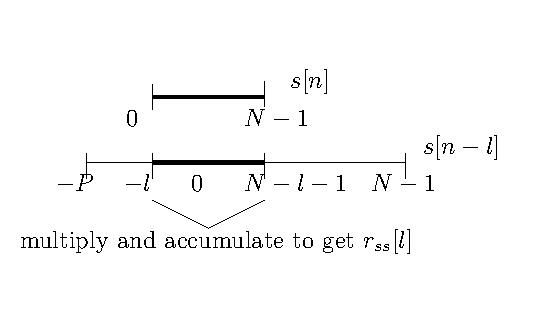
\epsfig{file=correlation.eps,width=6cm}
      \vspace*{0.5cm}
      \caption{Computing the autocorrelation coefficients}
      \label{fig:correlation}
   \end{center}
\end{figure}

Another related method of measuring the redundancy in a signal is to 
compute its autocovariance
\begin{equation}
        r_{ss}(l) = \frac{1}{N-l}\sum_{n=l}^{N-1}s(n)s(n-l)
\label{equ:autocovariance}
\end{equation}
where the summation is over $N-l$ products (the samples 
$s(-P),\ldots,s(-1)$ are ignored).
%It is known that for speech 
%signals, using the autocovariance coefficients has better stability for 
%linear prediction.

\subsection{Linear Prediction Model}
Linear prediction is a good model for recognition of 
speech signals.  In linear prediction, the human vocal tract 
is modeled as an infinite impulse respone (IIR) system that produces 
the speech signal.  For vowel sounds and other voiced regions of speech, 
which have a resonant structure and high degree of similiarity over 
particular time shifts, this modeling produces an efficient 
representation of the sound.  Figure \ref{fig:lpc model} shows how the 
resonant structure of a vowel could be captured by an IIR system.

\begin{figure}[htb]
  \begin{center}
      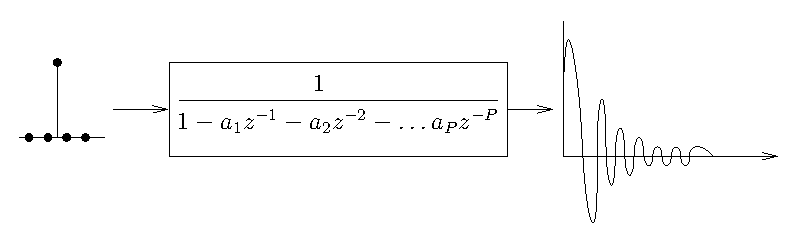
\epsfig{file=lpc_model.eps,width=12cm}
      \vspace*{1.5cm}
      \caption{Linear Prediction (IIR) Model of Speech}
      \label{fig:lpc model}
  \end{center}
\end{figure}


The linear prediction problem can be stated as finding the 
coefficients $a_k$ which result in the best prediction (which minimizes 
mean-squared prediction error) of the speech sample $s(n)$ in terms of 
the past samples $s(n-k)$, $k=1,\ldots,P$.  The predicted sample 
$\hat{s}(n)$ is then given by \cite{Rabiner}
\begin{equation}
        \hat{s}(n) = \sum_{k=1}^{P} a_k s(n-k)
\label{equ:prediction}
\end{equation}
where $P$ is the number of past samples of $s(n)$ which we wish to
examine.  Now, we derive the frequency response 
of the system in terms of the prediction coefficients 
$a_{k}$ as follows.  In (\ref{equ:prediction}), when the predicted sample 
equals the actual signal (i.e $\hat{s}(n) = s(n)$), we have
\begin{eqnarray}
        s(n) & = & \sum_{k=1}^{P} a_k s(n-k)    \nonumber \\
        S(z) & = & \sum_{k=1}^{P} a_k S(z)z^{-k}    \nonumber \\
        S(z) & = & \frac{1}{1 - \sum_{k=1}^{P}a_{k}z^{-k}}
\label{equ:IIR}
\end{eqnarray}
The optimal solution to this problem is \cite{Rabiner}
\begin{eqnarray}
        {\bf a} & = & \left[a_1 \,\, a_2 \,\, 
                        \ldots \,\, a_P \right] \nonumber \\
        {\bf r} & = & \left[r_{ss}(1)\,\, r_{ss}(2) \,\, 
                        \ldots \,\, r_{ss}(P) \right]^{T} \nonumber \\
        {\bf R} & = & \left(\begin{array}{c c c c c c}
        r_{ss}(0) & r_{ss}(1) & \ldots & r_{ss}(P-1) \nonumber \\ 
        r_{ss}(1) & r_{ss}(0) & \ldots & r_{ss}(P-2)  \nonumber \\
        & & \vdots \nonumber \\
        r_{ss}(P-1) & r_{ss}(P-2) & \ldots & r_{ss}(0) \nonumber \\
        \end{array}\right) \nonumber \\
        {\bf a} & = & {\bf R}^{-1}{\bf r}
\end{eqnarray}
Due to the Toeplitz property (symmetric with 
equal diagonal elements) of the ${\bf R}$ matrix, an efficient 
algorithm is available for computing ${\bf a}$ without finding 
${\bf R}^{-1}$.  Levinson's algorithm is an iterative method of 
computing the predictor coefficients ${\bf a}$ \cite{Rabiner} (p.115).

\vspace*{0.5cm}
\begin{tabular}{l l l}
Initial Step  &: $E_{0} = r_{ss}(0), i=1$\\
for i := 1 to P \{ \\
       &Step 1&: $k_{i} = \frac{1}{E_{i-1}}\left( r_{ss}(i) - 
                \sum_{j=1}^{i-1}\alpha_{j,i-1}r_{ss}(i-j) \right)$ \\ 
       &Step 2&: $\alpha_{j,i} = \alpha_{j,i-1} - k_{i}
                                  \alpha_{i-j,i-1}\,\,\,  
                                                j =1,\ldots,i-1$\\
       &     &\,\, $\alpha_{i,i} = k_{i}$\\
       &Step 3&: $E_{i} = (1-k_{i}^2)E_{i-1}$\\ 
\}
\end{tabular}
\vspace*{0.5cm}

\subsection{LPC-based Synthesis (Optional)}
Use the prediction coefficients to synthesize the original sound by 
applying $\delta(n)$, the unit impulse, to the IIR system with 
lattice coefficients $k_{i}$, $i=1,\ldots,P$ as shown in 
Figure \ref{fig:lattice}.  Apply 
$\delta(n)$ to consecutive IIR systems (which represent consecutive 
speech segments) to get a longer segment of synthesized speech.  

In this application, lattice filters are used rather than 
direct-form filters since they provide a good representation of 
the reflections in the vocal tract.  Lattice filters have 
coefficients with magnitude less than $1$ and are available 
directly as a result of the Levinson-Durbin algorithm.  If a 
direct-form implementation is desired, the $\alpha$ coefficients 
would need to be factored into second-order stages with 
very small gains to yield a more stable implementation.

\begin{figure}[ht]
   \begin{center}
      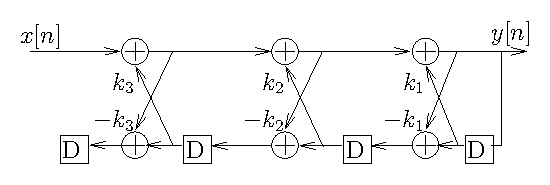
\epsfig{file=lattice.eps,width=9cm}
      \vspace*{0.5cm}
      \caption{IIR lattice filter implementation.}
      \label{fig:lattice}
   \end{center}
\end{figure}

When each segment of speech is synthesized in this manner, two problems 
occur.  First, the resulting synthesis is monotone and contains no 
changes in pitch since the $\delta(n)$ are input with the fixed 
periodicity equal to the segment length.  Second, the states of the 
lattice filter (values in the delay boxes) are cleared at the 
beginning of each segment, causing discontinuity in the output.

To recover the pitch, we look at the autocorrelation coefficients of 
each segment.  A large peak in the autocorrelation coefficient at 
lag $l\neq0$ would correspond to a periodicity $l$ of the speech 
in that segment.  If the speech segment does not have a large peak 
in the autocorrelation coefficients, then the segment is an 
unvoiced signal which has no periodicity.  Unvoiced segments such as 
consonants are best reconstructed by inputting noise into the IIR 
model.  For voiced segments such as vowels, an impulse train 
with delay between impulses varied according to the pitch period 
in each segment provides a good approximation to the originial pitch 
variation.

To reduce the discontinuity between segments, do not clear the 
states of the IIR model from one segment to the next.  Instead, load 
the new set of reflection coefficients, $k_i$, and continue with the 
lattice filter computation.

\begin{thebibliography}{2}

\bibitem{Proakis}
J.~G. Proakis and D.~G.Manolakis, {\em Digital Signal Processing: 
Principles, Algorithms, and Applications}.
\newblock Upper Saddle River, NJ: Prentice-Hall, 1996.

\bibitem{Rabiner}
L.Rabiner and B.-H. Juang, {\em Fundamentals of Speech Recognition}.
\newblock Englewood Cliffs, NJ: Prentice-Hall, 1993.

\end{thebibliography}

